\vspace{10pt}

{\centering\subsection*{何宇州:落日即景}}

\addcontentsline{toc}{subsection}{何宇州:落日即景}

\renewcommand{\leftmark}{何宇州:落日即景}

\begin{figure}[htbp]

\centering

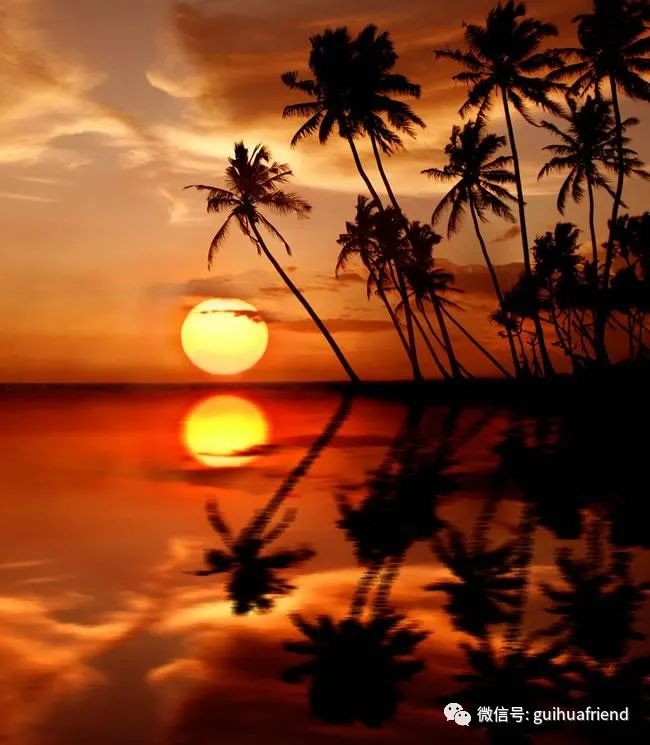
\includegraphics[width = .5\textwidth]{./ch/35.jpg}

\end{figure}



每个人都有自己喜欢的景物,而我喜欢日落时的景物。



下午的时候太阳公公收起中午时那耀眼的光芒,变成了一个红彤彤的大火球,像极了一个喝醉的人的脸蛋。夕阳落在窗户上,窗户好像被镶上了一抹金,一栋栋楼房金光闪闪,多么像一个个长方形的金色镜子。

过了一会儿,太阳公公在我们不注意的时候,变成了一个害羞的小姑娘,只剩下半边脸了,可是也掩盖不了那它那活泼好动的性格,太阳姑娘它也是很爱美的,她穿上五颜六色的云朵衣服。红色的地方就像一颗一颗颗美丽的红宝石,白色的地方就像一只小绵羊,它好像在对我们“咩咩”叫。蓝色的地方,好像是汹涌澎湃的海水。云朵有时候凑成一只凶猛的森林之王——老虎,那只老虎正在天上咆哮。还有一些云朵变成了一群小绵羊,它们在安详的地吃着鲜嫩的草,突然有一些云快速的变成了一只饥饿的饿狼,然后向那一群小绵羊扑了过去,之后羊群中的羊四处逃窜,最后不知道去了哪里。

又过了一会儿,疲惫的小鸟飞回巢里,劳作许久的人们回到家中。太阳带走了天空中的最后一片云霞,天空渐渐地暗了下来,因为月亮姐姐已经醒了,它和星星弟弟们一起挂在暗黑的天空中。





\vspace{10pt}



作者: 五(3)班 何宇州



指导老师:刘婷



投稿:2021年4月21日



发表:2021年4月27日






                



\vspace{10pt}

\hline



